\chapter{Face group fMRI data \label{Chap:data:faces_group}}

\section{Introduction}

These examples illustrate multisubject ``random effects'' analyses or ``second-level'' models of fMRI data \cite{will_hbf2_rfx}\footnote{This chapter has been largely cannibalised from an earlier document, available from \url{http://www.fil.ion.ucl.ac.uk/spm/data/face_rfx/spm2_face_rfx.doc}, which describes how to analyse this data using SPM2. That document additionally describes the analysis of differential effects, which we have omitted here.}.
The examples consist of three basic types of 2nd-level model:
\begin{enumerate}
\item \textbf{M2c:} Using contrast images for the canonical HRF only. This uses a single observation (contrast image) per subject only and data are analysed using a ``One-sample t-test''.
\item \textbf{M2i:} Using contrast images from an ``informed'' basis set, consisting of the canonical HRF and its two partial derivatives with respect to time (onset latency) and dispersion. This uses 3 observations (contrast images) per subject and data are analysed using a ``One-way ANOVA'' with 3 levels.
\item \textbf{M2f:} Using contrast images from a very general ``Finite Impulse Response'' (FIR) basis set, with 12 $\times$ 2 second timebins. This uses 12 observations (contrast images) per subject. Data are analysed using a ``One-way ANOVA'' with 12 levels.
\end{enumerate}

\section{Data}

The data come from the ``implicit'' condition of the Henson et al. study \cite{rnah_face_rep}. Although the 1st-level design matrices (and therefore resulting contrast images) used do not correspond exactly to those used in that study.

It is also the same study from which one subject is used to illustrate a single-subject fixed effects analysis (see chapter \ref{Chap:data:faces} in this manual).

Unlike the single-subject fixed effects example dataset, only two event-types were modelled: famous and nonfamous faces (initial and repeated presentations were collapsed together, as were correct and incorrect responses). Briefly, greyscale photographs of 52 famous and 52 nonfamous face were presented for 0.5s for fame judgment task (one of two right finger key presses). The minimal SOA (SOAmin) was 4.5s, with all faces randomly intermixed together with a further 52 null events (ie 2/3 probability of a face every SOAmin).

Original images were continuous EPI (TE=40ms,TR=2s) 24 descending slices (64$\times$64 3$\times$3 mm$^2$), 3mm thick, 1.5mm gap.

2nd-level models \textbf{M2c} and \textbf{M2i} derive from a 1st-level model (\textbf{M1i}), in which the events were modelled with Nf=3 basis functions: the canonical HRF, its partial derivative with respect to onset latency (``temporal derivative'') and its partial derivative with respect to dispersion (``dispersion derivative'').

2nd-level model \textbf{M2f} derives from an alternative 1st-level model (\textbf{M1f}), in which the same events were modelled with Nf=12 basis functions instead: corresponding to 2s timebins from 0-24s poststimulus (SPM's ``Finite Impulse Response'' or FIR basis set).

In both first-level models (\textbf{M1i} and \textbf{M1f}), the contrast images (\texttt{con*.img}'s) come from session-specific contrasts within a large (multisession) 1st-level Fixed Effects design matrix, with one session per subject. (Note that the resulting \texttt{con*.img}'s could equally well have been produced from 12 separate 1st-level models, one per subject.)

For each type of model, the main effect of faces versus baseline (eg, a [0.5 ... 0.5] contrast for each basis function, or \texttt{kron([0.5 0.5],eye(Nf))} more generally) was examined.

The 12 (subjects) \texttt{con*.img}s from the 1st-level model using the canonical HRF (\textbf{M1c}) are in the zipped file
\begin{itemize}
\item \url{http://www.fil.ion.ucl.ac.uk/spm/data/face_rfx/cons_can.zip}
\end{itemize}

The 12 (subjects) x 3 (basis functions) \texttt{con*.img}s from the 1st-level model using the informed basis (\textbf{M1i}) set are in the zipped file
\begin{itemize}
\item \url{http://www.fil.ion.ucl.ac.uk/spm/data/face_rfx/cons_informed.zip}
\end{itemize}

The 12 (subjects) x 12 (basis functions) x 2 (contrast-types) \texttt{con*.img}s from the 1st-level model using the FIR basis (\textbf{M1f}) set are in the zipped file
\begin{itemize}
\item \url{http://www.fil.ion.ucl.ac.uk/spm/data/face_rfx/cons_fir.zip}
\end{itemize}

Each contrast-type is examined in a separate SPM analysis. This chapter just describes analysis of the main effect of faces versus baseline.
To analyse the data, first create a new directory \texttt{DIR} eg. \texttt{c:$\backslash$data$\backslash$face\_group}, in which to place the results of your analysis. Then create 3 subdirectories (i) \texttt{Canonical}, (ii) \texttt{Informed}, and (iii) \texttt{FIR}. 
As the analysis proceeds these directories will be filled with job-specification files, design matrices and estimated models.

\section{Canonical HRF}

For the main effect versus baseline, these happen to correspond to the contrast images numbered 3-14 in 1st-level model \texttt{M1i}, ie:

\begin{itemize}
\item \texttt{con\_0006.img}       (canonical HRF, subject 1)
\item \texttt{con\_0007.img}       (canonical HRF, subject 2)
\item ...
\item \texttt{con\_0017.img}       (canonical HRF, subject 12)
\end{itemize}
These images comprise the data for \texttt{M2c}, which is simply a ``One-sample t-test''. This can be implemented as follows.
\begin{itemize}
\item Start up \matlab\ and type \texttt{spm fmri} at the prompt
\item Press the ``Specify 2nd-level'' button. This will open the batch editor.
\item In the ``Design'', ``One-sample t-test'' option, select ``Scans''.
\item Choose ``Select Files'' and use the SPM file selector to choose contrast images 6 to 17.
\item Highlight ``Directory'', ``Select files'' and select the  subdirectory \texttt{canonical}, to place the design matrix in.
\item Save the job file as eg. \texttt{DIR/canonical.mat}.
\item Press the \texttt{Run} button (green arrow).
\end{itemize}

SPM will then show you the design matrix shown in Figure~\ref{t1}. This is simply a single column of 1's which will appear as a white box on a white background. This design is encoded in the \texttt{SPM.mat} file that is written to the output directory.
\begin{figure}
\begin{center}
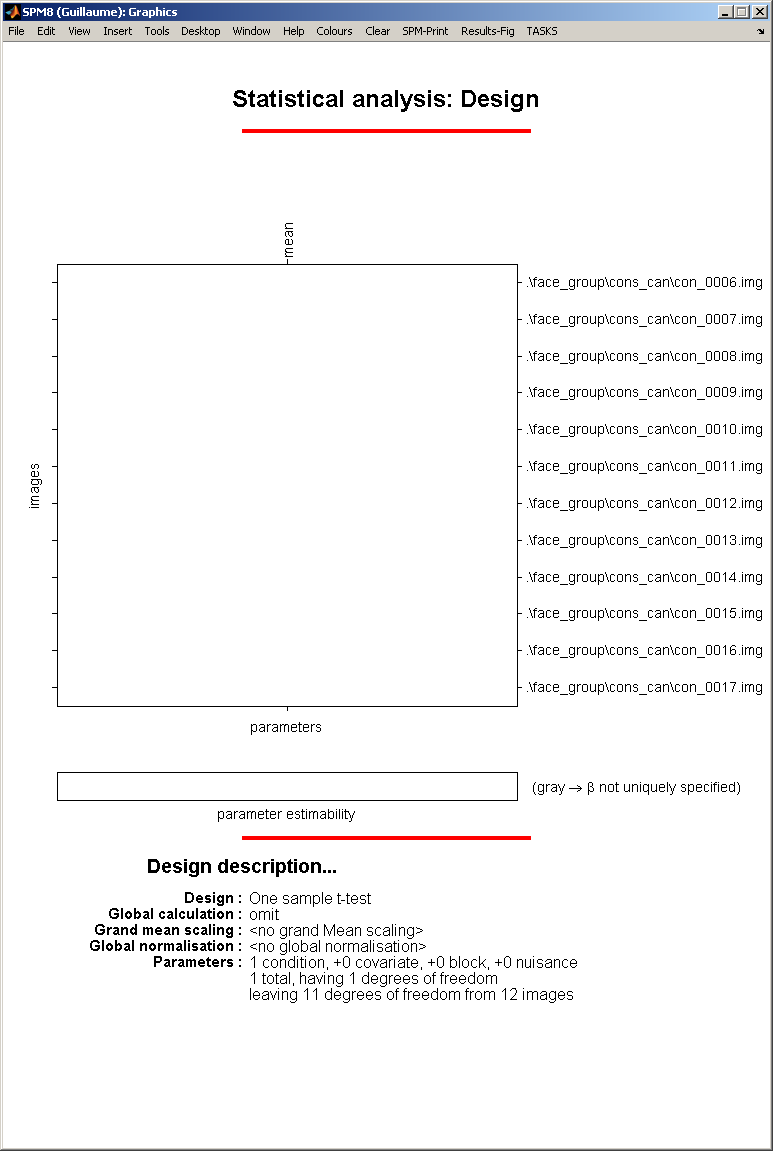
\includegraphics[width=140mm]{faces_group/t1}
\caption{\em \textbf{Design matrix for canonical responses}. This corresponds to a one-sample t-test. \label{t1}}
\end{center}
\end{figure}
Then press ``Estimate'', select the \textbf{SPM.mat} file just created, and press the \texttt{Run} button.
SPM will now estimate the parameters, that is, the size of the population effect at each voxel. This is simply the average of the \texttt{con*.img}s you have specified.

\begin{itemize}
\item Now press the ``Results'' button.
\item Select the \texttt{SPM.mat} file.
\item In the contrast manager press ``Define new contrast'' (select F). Enter [1] in the contrast section and enter ``Faces vs Baseline: Canonical HRF' as a ``name''. Note: This [1] F-contrast tests for both ``activations'' and ``deactivations'' versus the interstimulus baseline, though in the present case, the regions are nearly all activations, as can be seen by entering the same contrast weight [1], but as a T rather than F contrast.
\item Press the ``..submit'' button. Press OK.
\item Now press the ``Done'' button.
\item Mask with other contrast(s) [No]
\item Title for comparison: accept [Faces vs Baseline: Canonical HRF]
\item p value adjustment to control [FWE]
\item Family-wise p-value [0.05]
\item Extent threshold {voxels} [0]
\end{itemize}

SPM will now display the thresholded F-statistic image. This shows voxels that are significantly active (correcting for multiple comparisons across all voxels) in the population from which the subjects were drawn. They include bilateral posterior fusiform, SMA, and, at a more liberal threshold, left motor cortex). 
\begin{figure}
\begin{center}
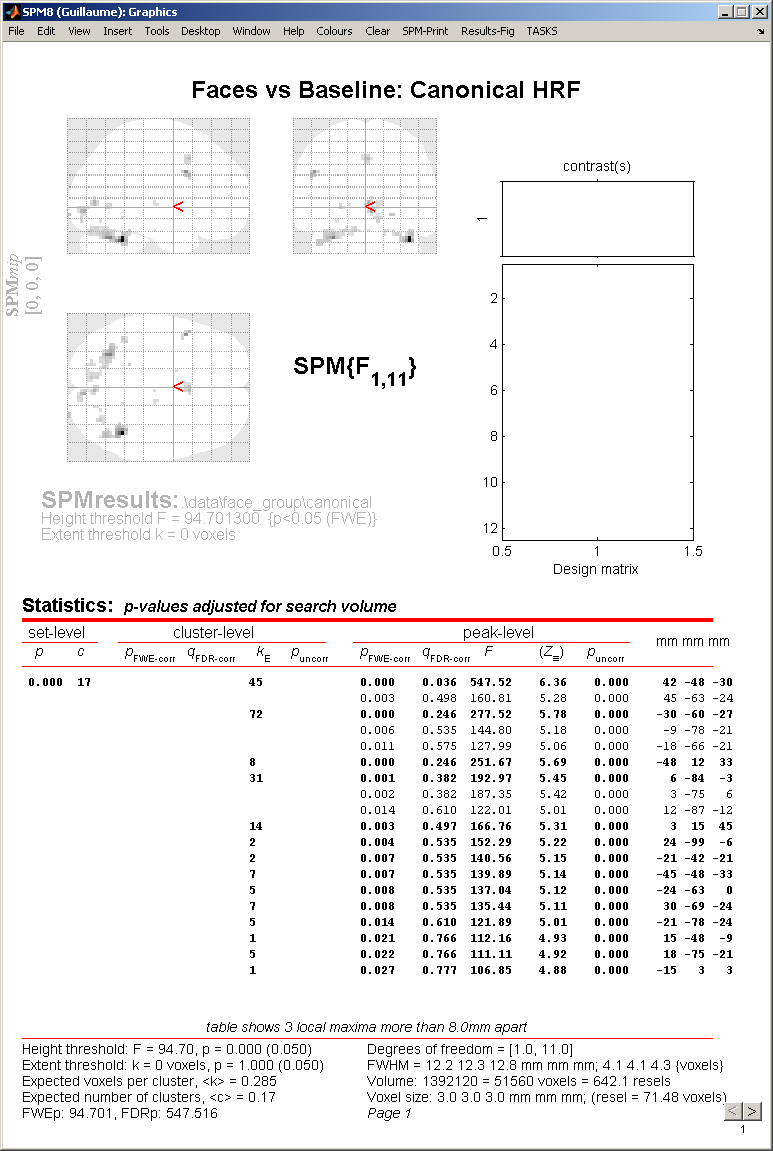
\includegraphics[width=140mm]{faces_group/f1_res}
\caption{\em Main population effect of faces vs baseline, as characterised using the Canonical HRF. \label{f1_res}}
\end{center}
\end{figure}
You can then press the volume to get a table of stastical information for clusters of activated voxels. SPM's graphics window should look like Figure~\ref{f1_res}.

\section{Informed basis set}

For this example, 3 contrast images per subject are taken to the 2nd-level. These are

\begin{itemize}
\item \texttt{con\_0003.img}       (canonical HRF, subject 1)
\item \texttt{con\_0004.img}       (canonical HRF, subject 2)
\item ...
\item \texttt{con\_0014.img}       (canonical HRF, subject 12)
\item \texttt{con\_0015.img}       (temporal derivative, subject 1)
\item \texttt{con\_0016.img}       (temporal derivative, subject 2)
\item ...
\item \texttt{con\_0026.img}       (temporal derivative, subject 12)
\item \texttt{con\_0027.img}       (dispersion derivative, subject 1)
\item \texttt{con\_0028.img}       (dispersion derivative, subject 2)
\item ...
\item \texttt{con\_0038.img}       (dispersion derivative, subject 12)
\item ...
\end{itemize}
These images comprise the data for \texttt{M2c}, which is simply a ``One-way ANOVA'' with 3-levels. This can be implemented as follows.
\begin{itemize}
\item Press the ``Specify 2nd-level'' button.
\item In ``Factorial design specification'', highlight ``Design'' and then choose ``Full Factorial''.
\item Under ``Factors'' create a single ``New Factor''.
\item In this ``Factor'', type in ``Basis'' for Name and enter 3 under ``Levels''.
\item Highlight ``Independence'' and select ``No''. SPM will then take into account possible correlations between these repeated measures (see section on Nonsphericity below for further discussion).
\item Now highlight ``Specify cells'', and create 3 new cells.
\item For the first cell, set ``Levels'' to \texttt{1}, and enter the canonical contrast images under scans (ie contrast images numbered \texttt{0003} to \texttt{0014}).
\item For the second cell, set ``Levels'' to \texttt{2}, and enter the temporal derivative contrast images under scans (ie contrast images numbered \texttt{0015} to \texttt{0026}).
\item For the third cell, set ``Levels'' to \texttt{3}, and enter the dispersion derivative contrast images under scans (ie contrast images numbered \texttt{0027} to \texttt{0038}.
\item Highlight ``Directory'', ``Specify files'' and select the subdirectory ``informed'', to place the design matrix in.
\item Save the job file as eg. \texttt{DIR/informed.mat}.
\item Press the \texttt{Run} button in the batch editor.
\end{itemize}

SPM will then show you the design matrix shown in Figure~\ref{informed_design}. This design is encoded in the \texttt{SPM.mat} file that is written to the output directory.
\begin{figure}
\begin{center}
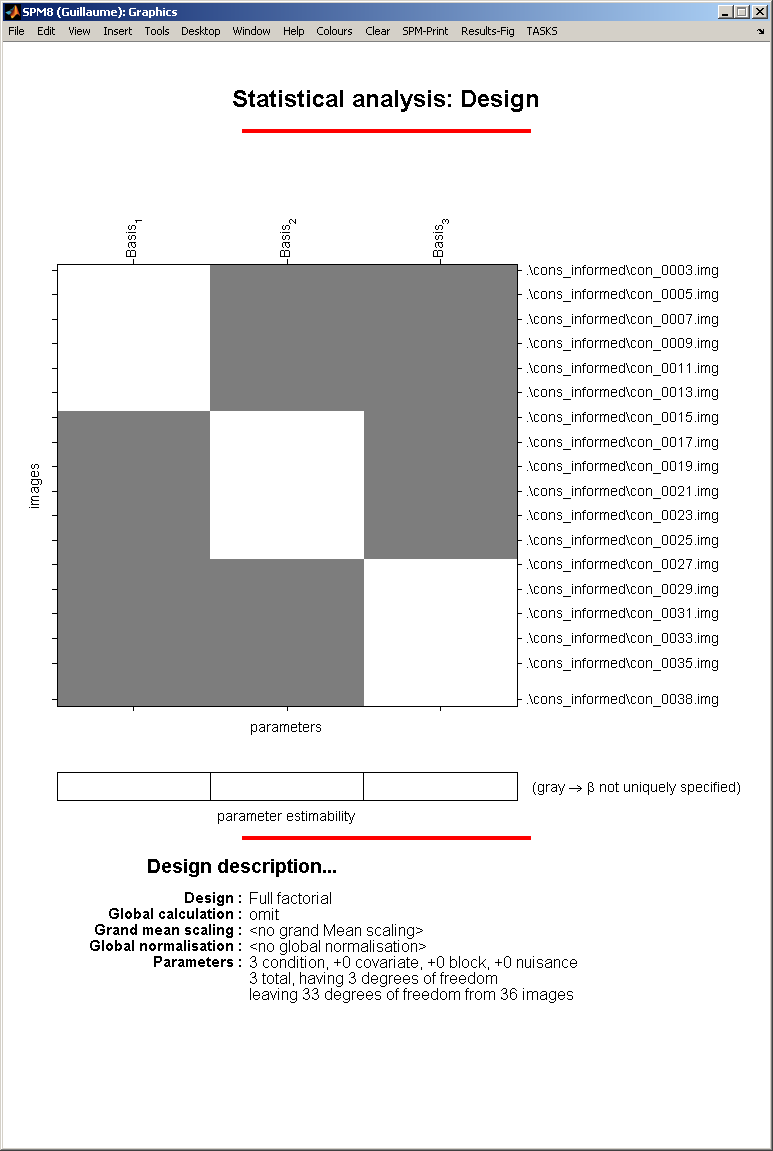
\includegraphics[width=140mm]{faces_group/informed_design}
\caption{\em \textbf{Design matrix for informed basis set.} This corresponds to a one-way ANOVA with three levels (but no constant term, since we want to test whether the basis functions are different from zero, not whether they are different from each other). \label{informed_design}}
\end{center}
\end{figure}
Then press ``Estimate'', select the \texttt{SPM.mat} file just created, and press the \texttt{Run} button.
SPM will now estimate the parameters of the model (and hyperparameters governing the nonsphericity).

\subsection{Nonsphericity}

Setting the independence option described above to ``No'' allows SPM to take into account possible correlations between levels of the factor. Note that, by default, SPM assumes different variances for different levels of the factor (you can change this by setting ``Variance'' to ``Equal'' under the options for the factor). 

In this way SPM can account for possible ``non-sphericity'' in the data. This is implemented in SPM using a set of matrices (bases) that characterise the covariance matrix. The first three correspond to the variance of each of the canonical, temporal and dispersion derivatives:  \texttt{SPM.xVi.Vi\{1\}}, \texttt{SPM.xVi.Vi\{2\}}, and \texttt{SPM.xVi.Vi\{3\}}.

The next three correspond to covariances: \texttt{SPM.xVi.Vi\{4\}} (covariance between canonical and temporal derivative), \texttt{SPM.xVi.Vi\{5\}} (covariance between canonical and dispersion derivative), and \texttt{SPM.xVi.Vi\{6\}} (covariance between temporal and dispersion derivatives).

After estimation the actual covariance values (hyper-parameters) are given by \texttt{SPM.xVi.h} (the six entries correspond to the above bases). The corresponding estimated covariance matrix can be shown by pressing Review$\rightarrow$Design$\rightarrow$Explore$\rightarrow$Covariance Structure. The estimated covariance for this data is shown in Figure~\ref{informed_covariance}.
\begin{figure}
\begin{center}
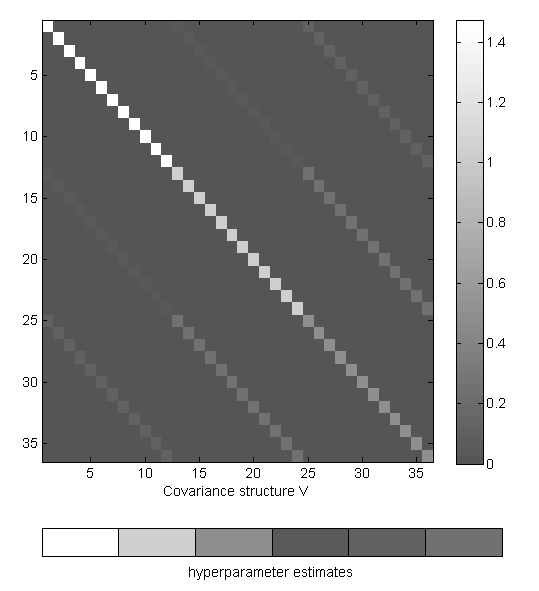
\includegraphics[width=100mm]{faces_group/informed_covariance}
\caption{\em \textbf{Estimated covariance matrix for informed basis set.} The 6 differently valued hyperparameters are shown in different shades of gray. \label{informed_covariance}}
\end{center}
\end{figure}
Note that these are ``global'' values which are scaled by a voxel specific-value to achieve a model covariance that best matches the empirical covariance at each voxel. 

\subsection{Informed Results}

\begin{itemize}
\item Now press the ``Results'' button.
\item Select the \texttt{SPM.mat} file.
\item In the Contrast Manager press ``Define new contrast'' (select F). Enter \texttt{eye(3)} in the contrast section and enter ``Faces vs Baseline: Informed'' as a ``name''. Note: In \matlab\ \texttt{eye(3)} evaluates to the identity matrix [1 0 0; 0 1 0; 0 0 1].\footnote{SPM will have produced some contrasts automatically, one of them being the ``main effect of basis''. This contrast is, however, not appropriate for our purposes.}
\item Press the ``..submit'' button. Press OK.
\item Now press the ``Done'' button.
\item Mask with other contrast(s) [No]
\item Title for comparison: accept [Faces vs Baseline: Informed]
\item p value adjustment to control [FWE]
\item Family-wise p-value [0.05]
\item Extent threshold {voxels} [0]
\end{itemize}

This contrast will reveal voxels that show some form of event-related response that can be captured by (ie, lies in the space spanned by) the three basis functions (e.g, 30 -60 -27, Z=7.43), as shown in Figure~\ref{informed_results}.
\begin{figure}
\begin{center}
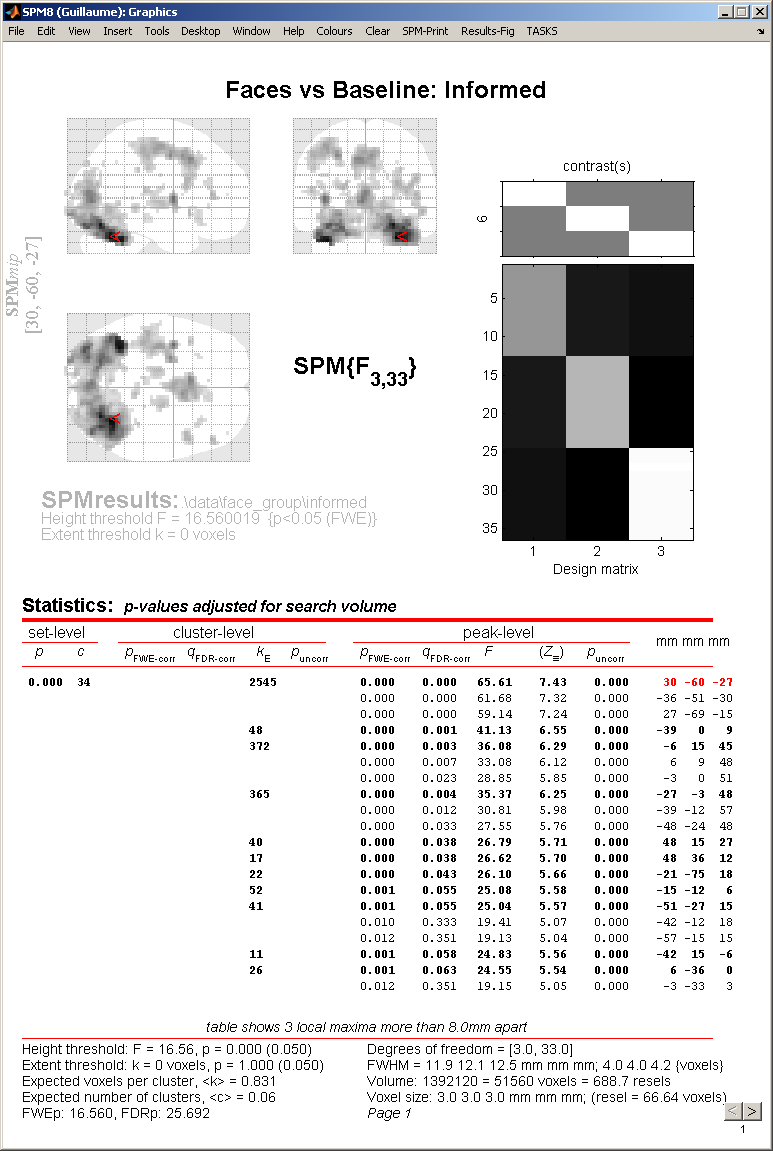
\includegraphics[width=100mm]{faces_group/informed_results}
\caption{\em Main population effect of faces, as characterised with the informed basis set. \label{informed_results}}
\end{center}
\end{figure}

Note how the design matrix appears to be different after estimation. This is because it has been pre-whitened (via the estimated nonsphericity). In particular, the (barely visible) off-diagonal entries in the design matrix give an indication of the degree of correlation between the basis functions across subjects. However, because the data have also been pre-whitened our interpretation of the parameter estimates (the ``betas'') is unchanged. Effectively the parameters have been estimated using ``Weighted Least Squares (WLS)'', where the weights relate to the estimated error covariance structure. SPM implements WLS by pre-whitening the data and the design matrix and then using ``Ordinary Least Squares'' (OLS).

Note also how this F-contrast (Figure~\ref{informed_results}) produces more significant results than the corresponding F-contrast in the model with the canonical HRF shown in Figure~\ref{f1_res}. This suggests significant additional information in the two derivatives of the canonical HRF. If you right-click on the MIP and select ``goto global maxima'', then press ``plot'', select ``Contrast estimates and 90\% C.I.'', and select the ``Faces vs Baseline: Informed'' contrast, you will get three bars and their confidence intervals, as in Figure~\ref{informed_plot}. You can see that the canonical HRF (first bar) carries most of the response vs baseline, but nonetheless, both the temporal and dispersion derivatives (second and third bars) contribute significant additional effects (given that the error bars do not overlap zero). Note that the size of the bars cannot be compared directly since they depend on the (different) scaling of the three basis functions (their size RELATIVE TO the error bars is a fairer way to compare the contributions of the different basis functions).

\begin{figure}
\begin{center}
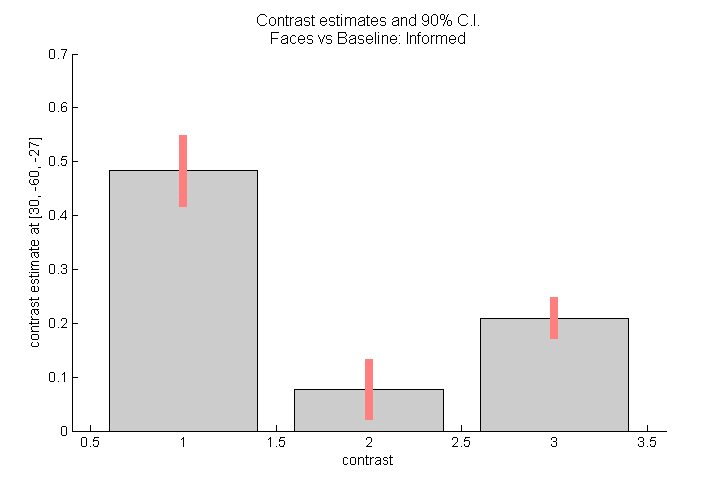
\includegraphics[width=100mm]{faces_group/informed_plot}
\caption{\em Plotting the three basis functions for the global maximum showing reliable effects of the canonical HRF and its time and dispersion derivatives. \label{informed_plot}}
\end{center}
\end{figure}

\subsection{T- and F-contrasts}

It is also informative to evaluate the T-contrast [1 0 0] (ie positive loadings on the canonical HRF only). This is shown in Figure~\ref{informed_t}.

\begin{figure}
\begin{center}
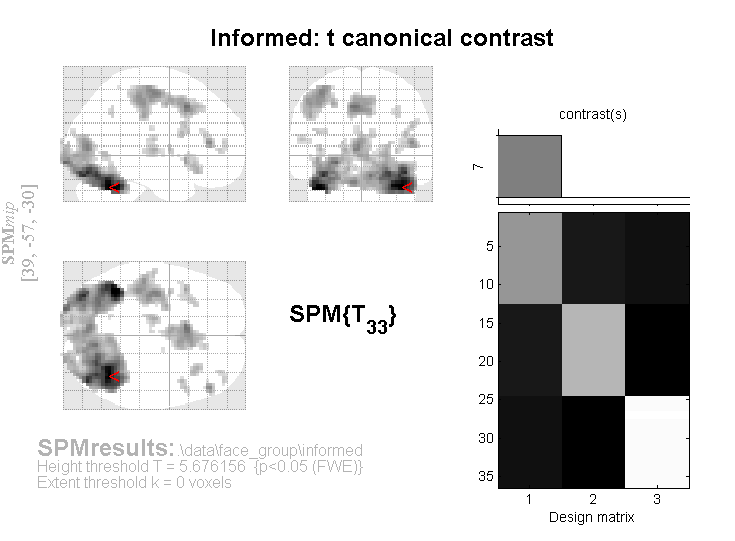
\includegraphics[width=100mm]{faces_group/informed_t}
\caption{\em Main population effect of faces, as characterised with the canonical HRF using a [1 0 0] t-contrast on the informed basis coefficients. \label{informed_t}}
\end{center}
\end{figure}
At a FWE correct p-value of 0.05, note more voxels (including now left motor cortex) and higher Z-values (e.g, 39 -57 -30, Z=7.53) for this main effect vs baseline compared to the equivalent T-contrast ([1]) in the model that uses only the canonical HRF (as in previous Section). 
The main reason for this increased power is the increase in the degrees of freedom, which entails better estimators of the underlying error (co)variance. The price of this increased power is a stronger assumption about the nonsphericity, namely that it has the same structure across (activated) voxels - the ``pooling device'', see Glaser et al. (2003) \cite{daniel_hbf2}.

\begin{figure}
\begin{center}
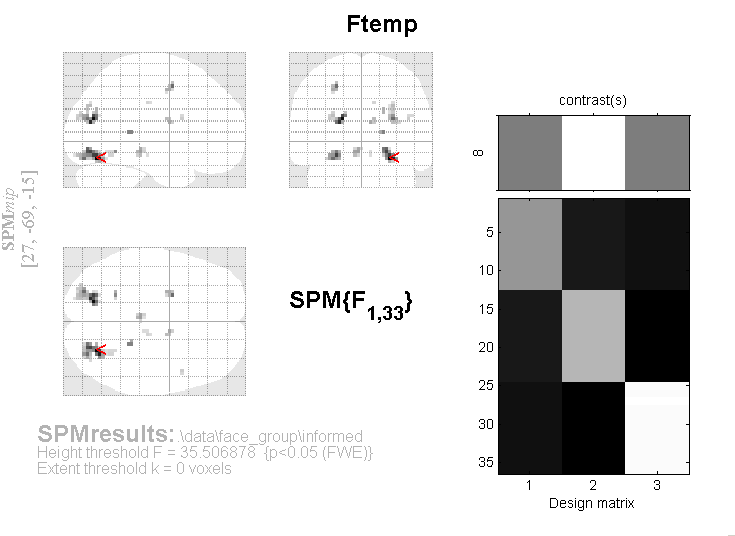
\includegraphics[width=100mm]{faces_group/Ftemp}
\caption{\em Significantly non-zero temporal derivative coefficients. These voxels show responses earlier or later than canonical responses. \label{informed_Ftemp}}
\end{center}
\end{figure}
\begin{figure}
\begin{center}
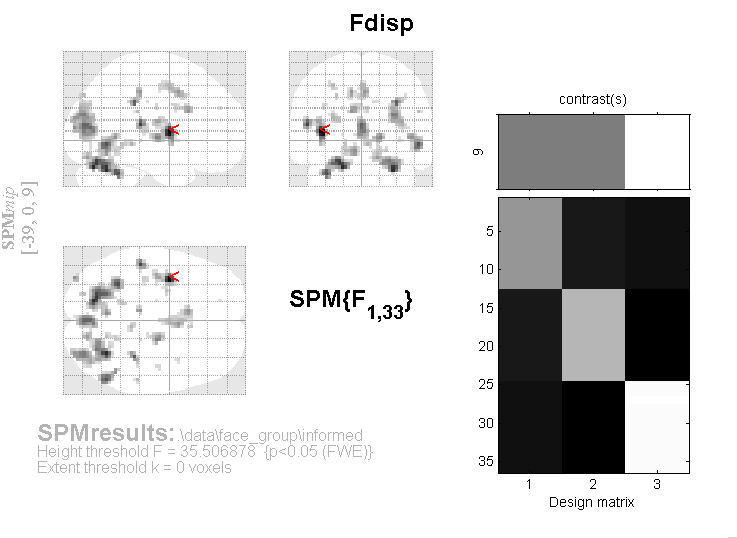
\includegraphics[width=100mm]{faces_group/Fdisp}
\caption{\em Significantly non-zero dispersion derivative coefficients. These voxels show responses narrower or wider than canonical responses. \label{informed_Fdisp}}
\end{center}
\end{figure}

Finally, evaluate the F-contrasts [0 1 0] and [0 0 1]. These are shown in Figures~\ref{informed_Ftemp} and~\ref{informed_Fdisp}.
These contrasts reveal voxels that load (positively or negatively) on the temporal and dispersion derivatives respectively. These contrasts reveal that there is significant variability (at p$<$.05 corrected) that is not captured by the canonical HRF alone (see below for more discussion; see also to Henson et al (2000) \cite{rnah_basis}.

In other words, some regions have earlier or later, or wider or narrower, BOLD impulse responses than the canonical HRF. This may reflect differences in vasculature (or even face-related neural differences across regions).  

On the other hand, note that most voxels in the above F-contrasts also show a positive loading on the canonical HRF (ie the previous [1 0 0] T-contrast), as can be revealed by Inclusive (or Exclusive) masking of the relevant contrasts. This is because the loadings on the derivatives reflect deviations ABOUT the canonical form (via a first-order Taylor expansion; see eg. Henson et al, 2002 \cite{rnah_latency}). Indeed, loadings on either derivative in the absence of a reliable loading (positive or negative) on the canonical HRF would be difficult to interpret (i.e, the derivative waveforms are probably too high frequency to reflect BOLD changes on their own).   

One can also confirm this by going to various voxels in the above F-contrasts, pressing ``plot'', ``contrast estimates'' and selecting the ``Can+Tem+Dis'' F-contrast. The three bars indicate the loadings (and 90\% confidence intervals) on the three different basis functions. Note that a positive estimate for the temporal derivative corresponds to an earlier response than the canonical (and negative for later), while a positive estimate for the dispersion derivative corresponds to a narrower (less dispersed) response (and negative for wider).

\section{FIR basis set}

For this example, 12 contrast images per subject are taken to the 2nd-level. These are the contrast images:

\begin{itemize}
\item \texttt{con\_fir\_bin01\_sub01.img}    (FIR bin 1, subject 1)
\item \texttt{con\_fir\_bin01\_sub02.img}    (FIR bin 1, subject 2)
\item ...
\item \texttt{con\_fir\_bin02\_sub01.img}    (FIR bin 2, subject 1)
\item ...
\end{itemize}

These images comprise the data for \texttt{M2f}, which is simply a ``One-way ANOVA'' with 12-levels (one for each time-bin). This can be implemented as follows.
\begin{itemize}
\item Start up \matlab\ and type \texttt{spm fmri} at the prompt.
\item Press the ``Specify 2nd-level'' button.
\item The options for ``Factorial design specification''\footnote{In SPM2, this data was analysed using the ``One-way ANOVA without a constant'' design. This option is no longer available in SPM5, as one-way ANOVA's are considered as factorial designs with a single factor.} appear.
\item Highlight ``Design'' and then choose ``Full Factorial''.
\item Under ``Full Factorial'' and `Factors' create a single ``New Factor''.
\item In this ``Factor'', type in ``TimeBin'' for ``Name'' and enter 12 under ``Levels''.
\item Highlight ``Independence'' and select ``No''. SPM will then take into account possible correlations between these repeated measures.
\item Now highlight ``Specify cells'', and create 12 new cells.
\item For the first cell, set ``Levels'' to \texttt{1}, and enter the contrast images for time bin 1 under scans. This is most easily done by changing the filter to \texttt{.*fir\_bin01.*}.
\item For the second cell, set ``Levels'' to \texttt{2}, and, under scans, enter the contrast images for time bin 2 This is most easily done by changing the filter to \texttt{.*fir\_bin02.*}.
\item Similarly for Levels 3 to 12.
\item Highlight ``Directory'', ``Specify files'' and select the subdirectory \texttt{FIR}, to place the design matrix in.
\item Save the job file as eg. \texttt{DIR/fir.mat}.
\item Press the \texttt{Run} button in the batch editor.
\end{itemize}


SPM will then show you the design matrix shown in Figure~\ref{fir_design}. This design is encoded in the \texttt{SPM.mat} file that is written to the output directory.
\begin{figure}
\begin{center}
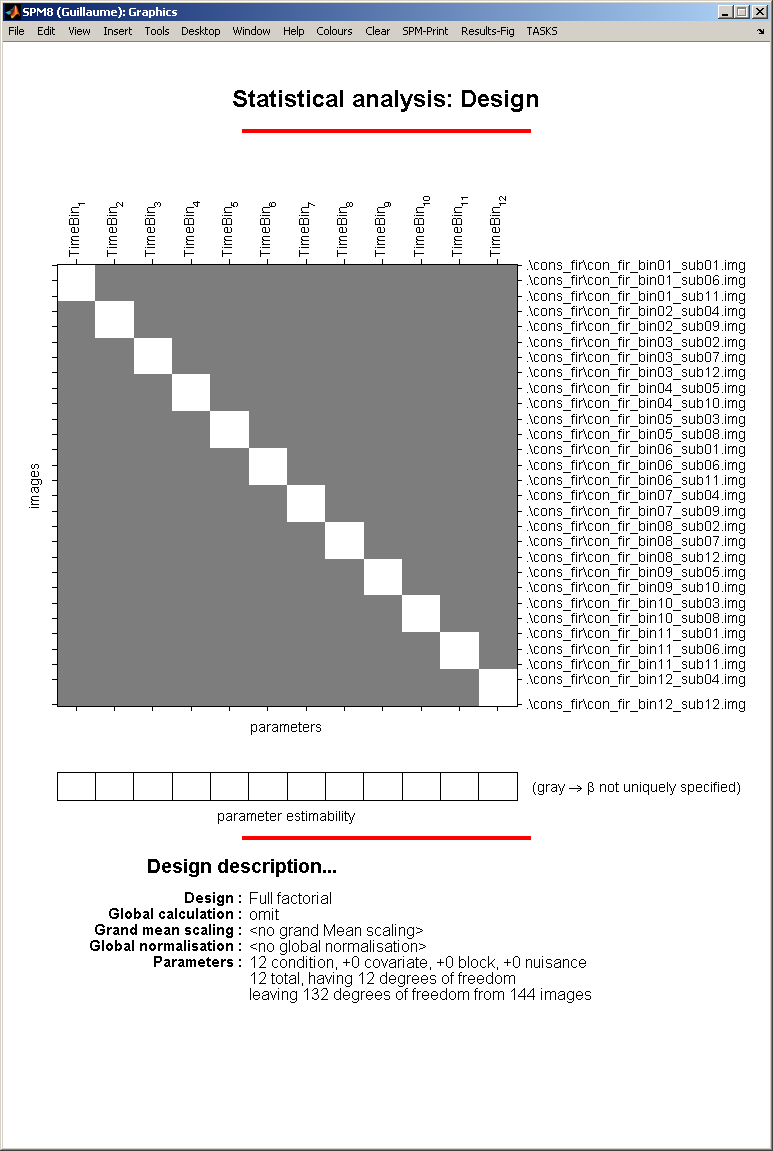
\includegraphics[width=100mm]{faces_group/fir_design}
\caption{\em Design matrix for FIR basis set. This corresponds to a one-way ANOVA with 12 levels. \label{fir_design}}
\end{center}
\end{figure}
Then press ``Estimate'', select the \texttt{SPM.mat} file just created, and press the button \texttt{Run}.
SPM will now estimate the parameters of the model.

\subsection{Nonsphericity again}

Setting the independence option to ``No'' allows SPM to take into account possible correlations between levels of the factor. Note that, by default, SPM assumes different variances for different levels of the factor (you can change this by setting ``Variance'' to ``Equal'' under the options for the factor). 

In this way SPM can account for possible ``non-sphericity'' in the data. This is implemented in SPM using a set of matrices (bases) that characterise the covariance matrix. The first 12 correspond to the variance of each of the responses in each of the 12 time bins. The ones that follow  correspond to covariances between different time bins.

After estimation the actual covariance values (hyper-parameters) are given by \texttt{SPM.xVi.h}. The corresponding estimated covariance matrix can be shown by pressing Review$\rightarrow$Design$\rightarrow$Explore$\rightarrow$Covariance Structure. The estimated covariance for this data is shown in Figure~\ref{fir_covariance}.
\begin{figure}
\begin{center}
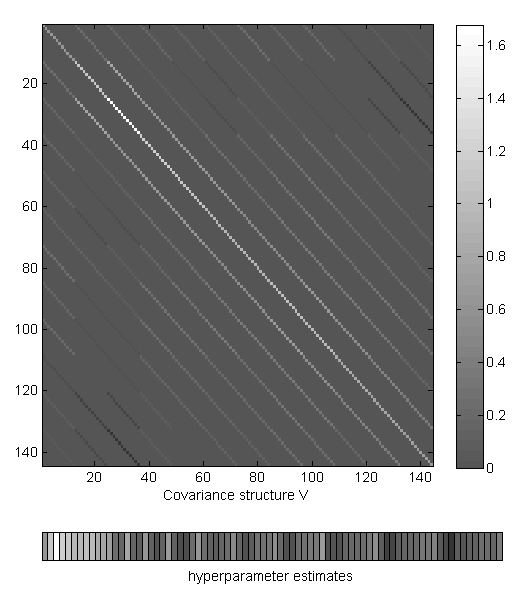
\includegraphics[width=100mm]{faces_group/fir_covariance}
\caption{\em Estimated covariance matrix for FIR basis set. The differently valued hyperparameters are shown in different shades of gray. Notice that the most variable responses occur in the third time bin (scans 25 to 36) corresponding to responses 4-6 seconds post stimulus, ie. at the peak of the hemodynamic response, as expected. \label{fir_covariance}}
\end{center}
\end{figure}
Note that these are ``global'' values which are scaled by a voxel specific-value to achieve a model covariance that best matches the empirical covariance at each voxel. 

You can see the highest values on the leading diagonal occur for timebins 2-4 (scans 13-48). This is where the peak response occurs, and the large values imply that, as expected, the variance tends to increase with the mean. This ``inhomogeniety of variance'' is a problem for conventional ANOVAs, but not here, where it is explicitly modelled.

Notice also the high values close to the diagonal, which reflect the positive correlation between the error across adjacent timebins (as also expected).

\subsection{FIR Results}

\begin{itemize}
\item Now press the ``Results'' button.
\item Select the \texttt{SPM.mat} file.
\item In the contrast manager press ``Define new contrast'' (select F). Enter \texttt{eye(12)} in the contrast section and enter ``Faces vs Baseline: FIR'' as a ``name'.\footnote{SPM will have produced some contrasts automatically, one of them being the ``main effect of TimeBin''. This contrast is, however, not 
appropriate for our purposes.}
\item Press the ``..submit'' button. Press OK.
\item Now press the ``Done'' button.
\item Mask with other contrast(s) [No]
\item Title for comparison: accept [Faces vs Baseline: FIR]
\item p value adjustment to control [FWE]
\item Family-wise p-value [0.05]
\item Extent threshold {voxels} [0]
\end{itemize}
Note how the design matrix, shown in Figure~\ref{fir_results} appears to be different after estimation. This is because it has been pre-whitened. In particular, the off-diagonal entries in the design matrix give an indication of the degree of correlation between the time bins across subjects (this is displayed explicitly in the covariance matrix in Figure~\ref{fir_covariance}).

The above contrast will reveal voxels that show \emph{any} form of event-related response, within the range 0-24s post-stimulus and with 2s resolution, as shown in Figure~\ref{fir_results}. 
\begin{figure}
\begin{center}
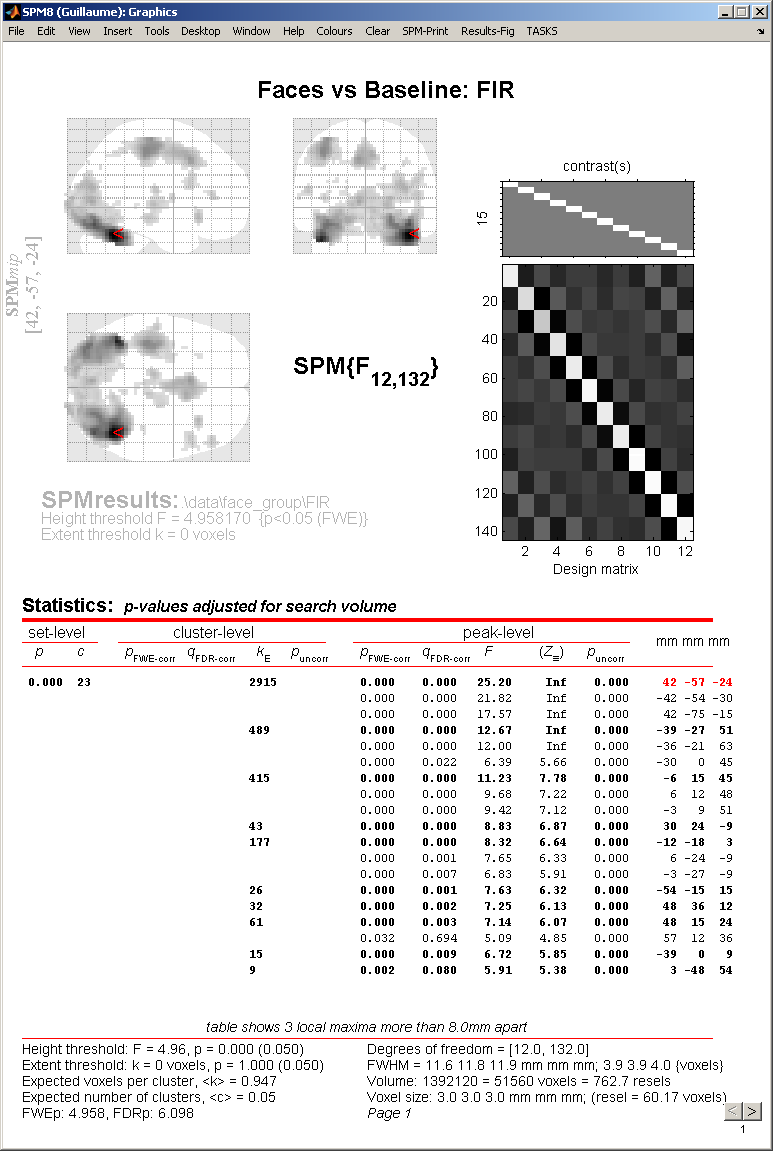
\includegraphics[width=100mm]{faces_group/fir_results}
\caption{\em Main population effect of faces, as characterised with the FIR basis set. \label{fir_results}}
\end{center}
\end{figure}
Selecting a voxel and plotting this contrast (using the \emph{plot} button) will reveal that most voxels have a fairly ``canonical'' shape over the 12 timebins.
One can also test for more constrained shapes of event-related responses within this model. For example, one can test for ``canonical-shaped'' responses by evaluating a contrast whose weights trace out SPM's canonical HRF (every 2s). To do this, switch to the \matlab\ window for a moment and type:
\begin{itemize}
\item \verb!xBF.dt = 1!
\item \verb!xBF.name = 'hrf (with time and dispersion derivatives)';!
\item \verb!xBF.length = 32;!
\item \verb!xBF.order = 1;!
\item \verb!xBF = spm_get_bf(xBF);!
\end{itemize}

This returns the canonical and two derivatives in the matrix \texttt{xBF.bf} (type \texttt{help spm\_get\_bf} for more info), with one value every 1 second. For convenience, then define:
\begin{itemize}
\item \verb!all     = xBF.bf(2:2:24,:)';!
\item \verb!can     = all(1,:);!
\item \verb!tem     = all(2,:);!
\item \verb!dis     = all(3,:);!
\end{itemize}

These commands downsample the basis functions every 2s, which is the bin-width of the FIR.
If you type \texttt{corrcoef(all')}, you will see that the basis functions are slightly correlated (in the off-diagonal terms), due to this undersampling every 2s.
\begin{itemize}
\item In the contrast manager press ``Define new contrast'' (select T).
\item Enter \texttt{can} as the contrast weights (defined in \matlab\ workspace as above), and ``Can-weighted FIR'' as the name.
\end{itemize}
This produces the MIP in Figure~\ref{can_weighted_fir}. At a FWE correct p value of 0.05, there are many more voxels compared to the equivalent T-contrast [1] in the model using only canonical HRF. The main reason for this increased power is again the increase in the degrees of freedom, which entails better estimators of the underlying error (co)variance (though if the FIR parameters were estimated very inefficiently, the extra contrast images might add more noise, outweighing any advantage of higher degrees of freedom). Again, this increased power comes with a stronger assumption about the nonsphericity, namely that it has the same structure across (activated) voxels \cite{daniel_hbf2}.
\begin{figure}
\begin{center}
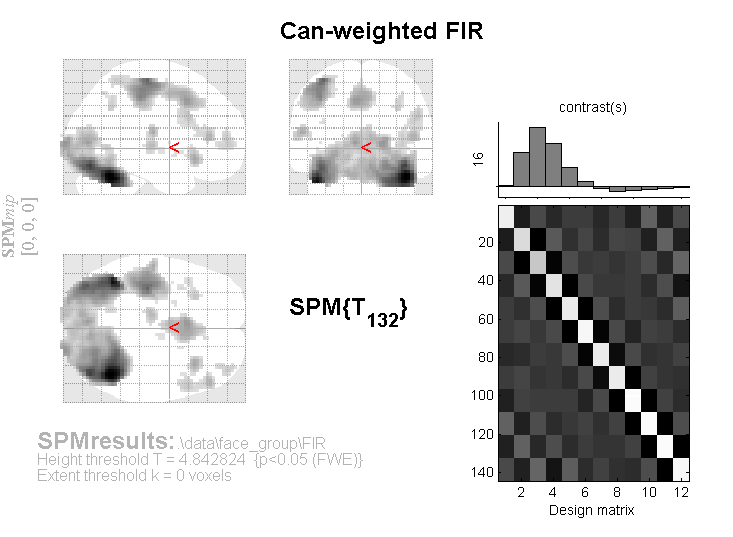
\includegraphics[width=100mm]{faces_group/can_weighted_fir}
\caption{\em Main population effect of faces, as characterised with a canonically weighted contrast of FIR bases. \label{can_weighted_fir}}
\end{center}
\end{figure}
One can also test the variance captured by the temporal and dispersion derivatives by creating new contrasts (though as F rather than T contrasts) and simply typing ``tem'' and ``dis'' respectively as the contrast weights.

More interesting is the ability to ask, within this model, how much event-related variance is \emph{not} captured by the canonical HRF. To do this, first create the variable in \matlab\:
\begin{itemize}
\item \verb!nullcan = eye(12) - pinv(can)*can;!
\end{itemize}

This creates a matrix for an F-contrast that spans the ``null space'' of the canonical HRF.
\begin{itemize}
\item In the contrast manager press ``Define new contrast'' (select F).
\item Enter \texttt{nullcan} as the contrast weights (defined in \matlab\ workspace as above), and ``Null space of canonical HRF'' as the name.
\end{itemize}

\begin{figure}
\begin{center}
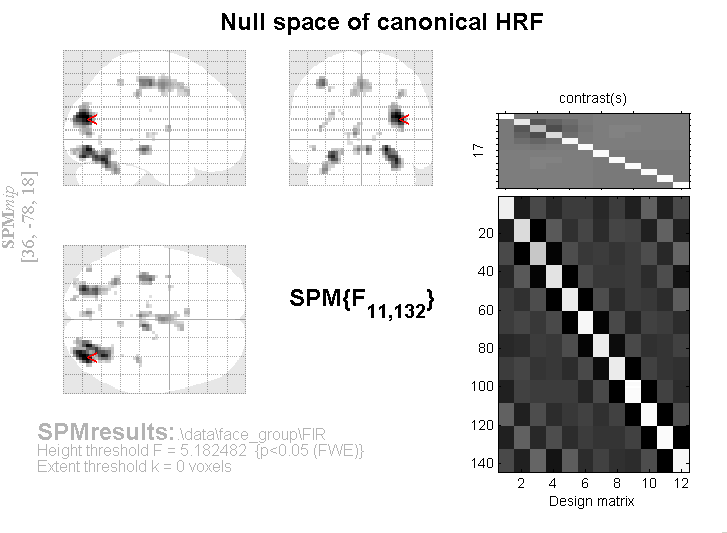
\includegraphics[width=100mm]{faces_group/nullcan}
\caption{\em Regions expressing variability across subjects not captured by canonical HRF. \label{nullcan}}
\end{center}
\end{figure}
You can see, in Figure~\ref{nullcan} that several regions express variability not captured by the canonical HRF. This is not surprising, because you will notice that many of these regions appeared in the individual F-tests on the temporal and dispersion derivatives above, suggesting that what is not captured by the canonical HRF is captured by its two derivatives.

Yet even more interesting is the ability to ask how much event-related variance is \emph{not} captured by the canonical HRF or its two derivatives (ie. not captured by SPM's `informed' basis set). To do this, first create the variable in \matlab\: 

\begin{itemize}
\item{\verb!nullall = eye(12) - pinv(all)*all;!}
\end{itemize}

This creates a matrix for an F-contrast that spans the ``null space'' of all three informed basis functions.
\begin{itemize}
\item In the contrast manager press ``Define new contrast'' (select F).
\item Enter \texttt{nullall} as the contrast weights (defined in \matlab\ workspace as above), and ``Null space of informed basis set'' as the name.
\end{itemize}

\begin{figure}
\begin{center}
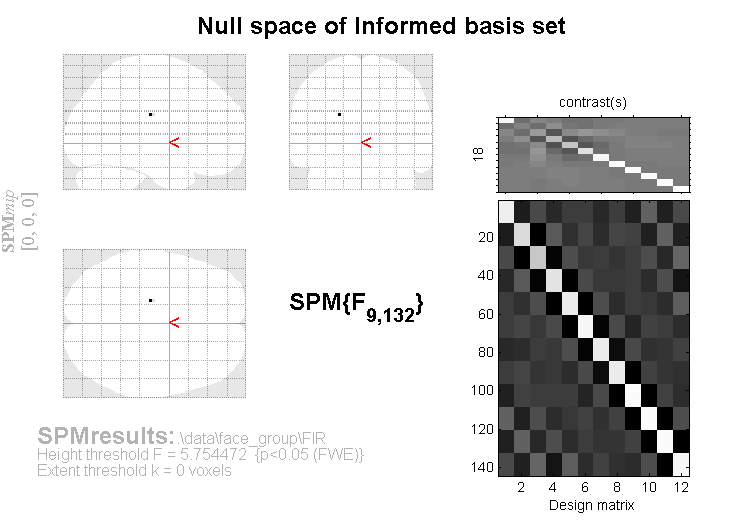
\includegraphics[width=100mm]{faces_group/nullall}
\caption{\em Regions expressing variability across subjects not captured by informed basis set. \label{nullall}}
\end{center}
\end{figure}
You will see, in Figure~\ref{nullall} that only 2 voxels (in one cluster with maximum -21 -18 27) express variability not captured by the informed basis set. This reinforces the point that, while there is certainly variability in the HRF across different brain regions, the canonical HRF and its two derivatives are sufficient to capture the majority of this regional variability (at least on average across the 12 subjects in this dataset). See \cite{rnah_basis} for further details.
